\documentclass[11pt,a4paper,twoside]{article}
\usepackage[T1]{fontenc}
\usepackage[utf8x]{inputenc}
\usepackage{latexsym,amsfonts,amsmath,amsthm,amssymb, mathrsfs}
\usepackage{xcolor,bm, bbm}
\usepackage{amssymb}
\usepackage{tikz}
\usepackage{pgfplots}
\usetikzlibrary{patterns}

\begin{document}

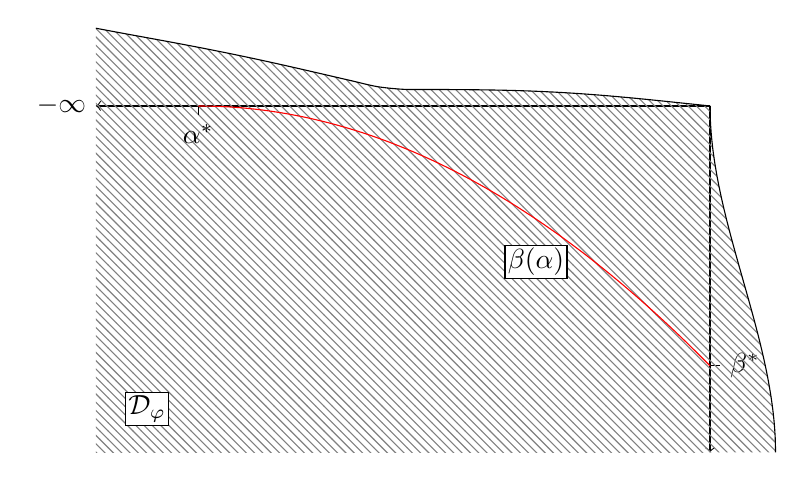
\begin{tikzpicture}[xscale=1.3, yscale=1.1]
    % Koordinatensystem
    \draw[<-] (-6,0) -- (0,0) node[left] {};
    \draw[->] (0,0) -- (0,-4) node[above] {};

    \fill[ pattern=north west lines, pattern color=gray] (-6,0) -- (0,0) -- (0,-4) -- (-6,-4) -- cycle;
    % Funktion

    % Achsenbeschriftungen
    \foreach \x in {-5}
        \draw (\x,0) -- (\x,-0.1) node[below] {$\alpha^*$};
        \draw (0,-3) -- (0.1,-3)
        node[right] {$\beta^*$};
        \draw (-1.7, -1.8) node[rectangle, draw, fill=white, inner sep=1pt] {$\beta(\alpha)$};
         \draw (-5.5, -3.5) node[rectangle, draw, fill=white, inner sep=1pt] {$\mathcal{D}_{\varphi}$};
        \draw[domain=-5:0,smooth,variable=\x,red] plot ({\x},{ -3/25*((\x+5)^2)}) node[right] {};
        \draw (-6,0) node[left] {$-\infty$};
        \fill [pattern=north west lines, pattern color=gray, domain=-6:0, variable=\x]
      (-6, 0)
      -- plot ({\x}, {0.15*(0.01*abs(\x)^3 + 0.1*(\x)^2 + 0.8*abs(sin(deg(\x))))})
      -- cycle;

       \draw[domain=-6:0,smooth,variable=\x,black] plot ({\x},{0.15*(0.01*abs(\x)^3 + 0.1*(\x)^2 + 0.8*abs(sin(deg(\x))))}) node[right] {};

      
       \fill [pattern=north west lines, pattern color=gray, domain=-4:0, variable=\x, rotate=90]
      (-4, 0)
      -- plot ({\x}, {-0.4*(-0.05*abs(\x)^3 + 0.3*(\x)^2 )})
      -- cycle;
      
      \draw[domain=-4:0,smooth,variable=\x,black, rotate=90] plot ({\x},{-0.4*(-0.05*abs(\x)^3 + 0.3*(\x)^2 )}) node[right] {};

\end{tikzpicture}

\end{document}